In this thesis, we leverage web technologies and standards to build interoperability in \ac{DTE}. 
Accordingly, this chapter provides an overview of the principal Web technologies, standards and architectural patterns and discuss how they build interoperability in heterogeneous systems. 
%
Additionally, we introduce the \ac{WoT} as an example of how web technologies can be applied in the \ac{IoT} context to achieve interoperability. 


%=======================================================
\section{History and Definitions}
%=======================================================


The World Wide Web, or simply, the Web, was initially proposed as an \emph{information management} system by Tim Berners-Lee in 1989 while working at CERN as a way to facilitate information sharing among researchers~\cite{berners1989information,Gillies_Cailliau_2000}.
%
The fundamental intuition of the Web is to apply the concept of \emph{hypertext}~\cite{nelson1967getting}---text containing links to other documents---to a global network of computers, enabling users to navigate and access information seamlessly across different systems through following Web links.
%
This allows to: 
\begin{itemize}
    \item easily add and link new information without requiring changes to existing systems;
    \item access and share information across a distributed network of computers in a location-independent manner.
\end{itemize}

The Web quickly evolved from a private information-sharing system, to a \emph{universe of global accessible information}~\cite{Berners-Lee_1996}
%
To implement this vision, the Web has been built on a set of fundamental building blocks: 
\begin{itemize}
    \item the \ac{URI} scheme for identifying resources on the Web;
    \item the \ac{HTTP} protocol for communication between clients and servers;
    \item the \ac{HTML} markup language for structuring and presenting information.
\end{itemize}
These essential Web architecture components are standardized by the \ac{W3C}, an international organization that maintains and develops open standards to ensure the long-term growth of the Web. The \ac{W3C} defines the Web as:

\begin{quote}
The World Wide Web (WWW, or simply Web) is an information space in which the items of interest, referred to as resources, are identified by global identifiers called \acfp{URI}~\cite{wwwarch2004}.
\end{quote}

The definition highlights the role of \emph{resources} as the first-class entities composing the Web. 
%
Resources can represent anything, from documents and images, to services, people and physical objects. 

The history of the Web is often divided into three main generations.
%
Web 1.0 refers to the early days of the Web, characterized by static web pages and limited interactivity.
%
In the early 2000s, the concept of Web 2.0 emerged to highlight the shift towards a more dynamic and interactive Web, in which users could not only consume content but also create and share it through social media, blogs, and wikis.
%
The third and current generation, Web 3.0, is often associated with the emergence of structured data, shifting the focus from human consumption to machine-readable representations~\cite{Aghaei_2012}.

The \emph{Semantic Web}~\cite{berners2023semantic} represents a vision for a Web of data that can be processed and understood by machines, enabling intelligent applications and services.
%
The Semantic Web builds on the existing Web infrastructure and introduces new standards and technologies to represent, share, and reason about data in a machine-readable way. 

\begin{figure}
    \centering
    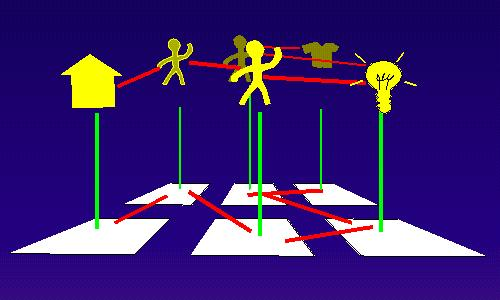
\includegraphics[width=0.8\textwidth]{figures/semantic.jpg}
    \caption{A slide showing the concept of the Semantic Web, with documents linked to real-world concepts through semantics, from \cite{bernerslee1994www94plenary}.}
    \label{fig:semantic-web-idea}
\end{figure}

In its keynote talk outlining future directions for the Web at the 1994 World Wide Web Conference, Tim Berners-Lee discussed the role of semantics on the Web (see \Cref{fig:semantic-web-idea}): 

\begin{quote}
But to a computer, it looks kind of flat [...] what it sees is a bunch of documents [...] and in fact we know that there is a world that is being described by these documents [...] but there is no semantics out there [...] the World Wide Web scaled, and it was sufficiently fun for everybody to use, but I missed out on putting semantics in [...] Semantics allow machines to manipulate reality. Well, machines at the moment can browse the Web, but if you put semantics over this then machines basically are browsing through reality~\cite{bernerslee1994keynote}.
\end{quote}

Following this original vision, in this thesis we leverage (semantic) Web technologies and standards to build interoperability in \ac{DTE}, with the goal of representing physical reality with machine-readable descriptions through networks of interconnected \acp{DT}.

%=======================================================
\section{The Web Architecture and Hypermedia}
%=======================================================

\todo{Maybe a figure of REST?}

The Web's success is a testament to how its design rationale, open standards, and protocols can enable seamless integration across diverse systems and data sources.
%
The architecture of the Web is based on a client-server model, where clients (e.g, web browsers) request resources from servers (e.g., web servers) using the \ac{HTTP} protocol.
%
This strong separation of concerns allows clients and servers to evolve independently, as long as they adhere to the same protocols and standards.
%
The principles of the Web architecture were formalized by Roy Fielding's PhD dissertation~\cite{fielding2000architectural}, where he introduced the concept of the \emph{\ac{REST}} architectural style.

\ac{REST} is defined by a set of constraints that promote scalability and interoperability in distributed systems. 
%
Constraints include client-server separation with stateless interactions for a strong separation of concerns, a \emph{uniform interface} between the two, cache mechanisms to improve performance and scalability supporting a layered system architecture, and code-on-demand for extensibility of client functionality~\cite{fielding2000architectural}.
%
The \emph{uniform interface} constraint is the cornerstone of \ac{REST}, achieved through:
\begin{itemize}
    \item resources identified by \acp{URI} which can unambiguously reference any entity in the global Web;
    \item manipulation of resources via a small set of methods (e.g., HTTP GET, PUT) for exchanging representations (e.g., JSON, XML) of their current or intended state; 
    \item self-descriptive messages using standard methods, media types, etc.;
    and
    \item server-guided navigation presenting both data and currently available controls using \ac{HATEOAS}.
\end{itemize}

The last point highlights the importance of \emph{hypermedia} in the Web architecture.
%
Although originally coined to extend the concept of hypertext to include multimedia content, Fielding defined hypermedia as:

\begin{quote}
Hypermedia is defined by the presence of application control information embedded within, or as a layer above, the presentation of information. Distributed hypermedia allows the presentation and control information to be stored at remote locations~\cite{fielding2000architectural}.
\end{quote}

This perspective shifts the focus from merely linking static documents to enabling dynamic interactions and navigation in the Web.
%
This makes the Web not only a repository of information but also an interactive platform for applications and services.
%
The Web's hypermedia nature, in fact, allows clients to discover and interact with resources dynamically, following links and controls provided by servers, rather than relying on fixed, predefined interactions.

The \ac{HATEOAS} sub-constraint of the uniform interface is particularly relevant for supporting the dynamic discovery of resources and actions in the open Web.
%
In a famous blog post, Fielding clarified the importance of \ac{HATEOAS}, explaining that hypermedia is the \emph{``simultaneous presentation of information and controls such that the information becomes the affordance through which the user (or automaton) obtains choices and selects action''}~\cite{fielding2008hypertext}.
%
The Web's hypermedia-driven interactions enable clients to navigate and interact with resources dynamically, following links and controls provided by servers, based on the current context and state of the application.
%
This mechanism further cements the Web as a platform for building interoperable systems that can evolve and adapt over time and that can support automated clients in discovering interactions and adapting to changes.

%=======================================================
\section{Semantic Web Technologies}
%=======================================================

The Semantic Web vision~\cite{berners2023semantic} exploits the hypermedia-based nature of the Web and advances interoperability by introducing machine-readable representations with shared semantics.
%
The Semantic Web is not ``a separate Web, but an extension of the current one''~\cite{berners2023semantic}, as such, it shares the same fundamental building blocks (e.g. \ac{URI}, \ac{HTTP}, \ac{REST}) and extends them with a set of dedicated standards and technologies to represent data in order to be processed and understood by machines.


\begin{figure}[ht]
    \centering
    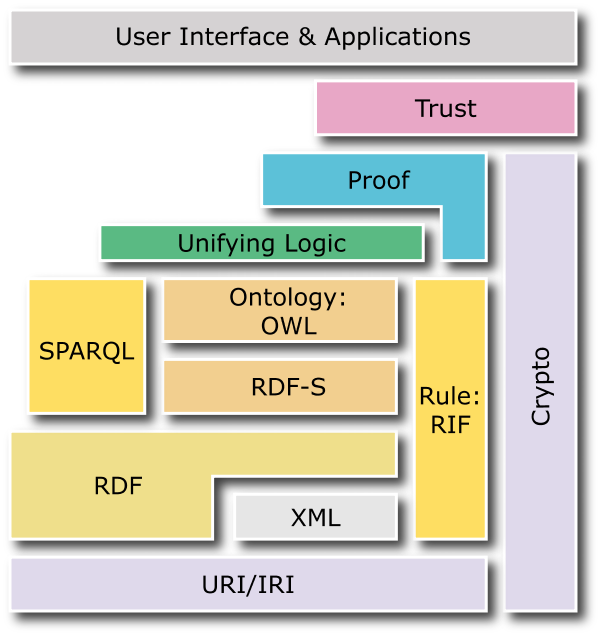
\includegraphics[width=0.8\textwidth]{figures/semantic-web-stack.png}
    \caption{The Semantic Web ``cake'' showing the layers of the technological stack, from \cite{bratt2007semanticweb}.}
    \label{fig:semantic-web-stack}
\end{figure}


\Cref{fig:semantic-web-stack} illustrates the layers of the Semantic Web technological stack with the main standards associated with each layer. 

The foundational building block is the \ac{RDF}, which provides a common data model for representing information about resources on the Web in the form of subject-predicate-object \emph{triples}~\cite{rdf-concepts}.
%
\ac{RDF} triples compose a directed labeled graph, where nodes represent resources and edges represent relationships between them. 
%
Nodes can be either \acp{IRI} (an extension of \acp{URI}) identifying a resource or \emph{literals} representing a typed value (e.g., string, number, date).
%
Additionally, \ac{RDF} supports \emph{blank nodes} to represent resources without a global identifier and support more complex structures than the basic triple structure allow.
%
In its latest version, \ac{RDF} officially supports also having \emph{triple terms} enabling the use of triples as objects of other triples, previously introduced by the {RDF-star} extension~\cite{hartig2021rdfstar}.
%
Predicates of a \ac{RDF} triples are always \acp{IRI}, which ensures a consistent and unambiguous identification of the relationships between resources.
%
Through the combination of these basic elements, \ac{RDF} enables the representation of relationships between resources, which can encode machine-understandable knowledge about a domain.

\ac{RDF} can be serialized in various formats, with the original being an XML-based syntax, while more recent formats include the JSON-LD syntax popular due to its compatibility with JSON-based systems~\cite{json-ld} and \emph{Turtle} syntax, which provides the most compact and human-readable representation of \ac{RDF} graphs~\cite{turtle}.


\todo{Example of RDF triples or figure??}

The next step in the Semantic Web stack is the introduction of vocabularies to provide shared semantics for the terms used in \ac{RDF} graphs.
%
This is essential to ensure that different systems can understand and interpret data with consistent meanings.
%
The concept of \emph{ontology}~\cite{Vickery_1997} is used to refer to a formal definition of concepts and relationships within a specific domain.

The basic vocabulary layer is provided by \ac{RDF} Schema~\cite{rdfs}, which introduces a simple set of terms to define classes and properties. 
%
The more expressive \ac{OWL}~\cite{olw2overview} builds on \ac{RDF} Schema to provide a richer set of modeling primitives.
%
Through \ac{OWL} ontologies, it is possible to establish taxonomies of concepts and inference rules that enable reasoning over the represented knowledge, as well as axioms that can be used to validate data against the defined schema and discover inconsistencies. 

The combination of \ac{RDF} triples and \ac{OWL} ontologies enables the creations of \emph{\acp{KG}}~\cite{KG_Book:21}, creating a structured representation of knowledge through the primitives provided by these standards.
%
\ac{KG} have the benefit of not requiring a predefined schema, creating a flexible and extensible representation of knowledge that can easily evolve over time. 

\todo{Example of SPARQL query?}

Accessing data in a \ac{KG} requires dedicated query languages that can traverse the graph structure and retrieve relevant information.
%
The \ac{SPARQL}~\cite{sparql} is the standard query language for \ac{RDF} data. It is designed to be SQL-like, making it familiar to use for developers used to relational databases.
%
\ac{SPARQL} allows the retrieval of data by matching graph patterns. The result of a query is a list of variable bindings that satisfy the specified pattern. 

The core set of standards presented above simply provides the foundations for the Semantic Web. 
%
Other relevant technologies include validation of \ac{RDF} data by means of matching \emph{shapes} and conditions using \ac{SHACL}~\cite{shacl}, and rule-based reasoning with \ac{SWRL}~\cite{swrl} which extend the inference capabilities of \ac{OWL} with Horn-clause rule logic~\cite{Horn_1951}.

Interestingly, the technologies described above, can be used outside the Web context, for example for building local \acp{KG} to serve as databases for specific applications. 
%
When integrated with the Web architecture and principles, however, they enable the creation of so-called \emph{Linked Data}~\cite{Bizer_Heath_Berners-Lee_2023}.
%
Originally proposed by Tim Berners-Lee in 2006~\cite{berners-lee2006linkeddata}, Linked Data is grounded on four main principles:
\begin{enumerate}
    \item User \acp{URI} as names for things;
    \item Use \ac{HTTP} \acp{URI} so that people can look up those names;
    \item When someone looks up a \ac{URI}, provide useful information, using the standards (e.g., \ac{RDF}, \ac{SPARQL});
    \item Include links to other \acp{URI} so that they can discover more things.
\end{enumerate}

Together, these principles promote the interrelation of \ac{RDF} resources, enabling the creation of a global distributed \ac{KG} that applications can navigate by following and dereferencing \ac{HTTP} \acp{URI}. 
%
In Linked Data, \acp{URI} are used not only to identify documents and web pages, but also real-world entities, concepts, and abstract ideas.
%
The disambiguation between information resources (e.g., documents) and non-information resources (e.g., people, places, physical objects) is achieved through the use of \emph{hash} or \emph{303} \ac{URI} patterns~\cite{cool-uris}.

To complete the consumption and interaction with Linked Data, the \ac{LDP} specification~\cite{ldp} defines rules and best practices on how to apply \ac{REST} principles to the management of \ac{RDF} resources.
%
\ac{LDP} servers expose \emph{containers} of \ac{RDF} resources, that clients can interact with using \ac{HTTP} methods to create, read, update and delete resources. Depending on the type of container, the containment relationship is implicitly or explicitly represented, to ease the discovery of related resources.

The combination of Semantic web technologies and Linked Data principles provides a powerful framework for creating distributed knowledge bases that can be easily shared, integrated and queried across different systems.
%
Of course, the adoption of this approach is not without challenges. 
%
Despite being around for over two decades, the Semantic Web is still far from the original vision of a global Web of data that can be easily consumed by machines~\cite{Hogan_2020}. 
%
Nevertheless, the technological standards and principles described above have been successfully applied and still offer a solid foundation for building open interoperable ecosystems in which data is shared and integrated with clear semantics, supporting automated reasoning and advanced analytics.

\todo{possibly discuss more about challenges and applications}

%=======================================================
\section{The \acl{WoT}}
%=======================================================

Among the domains in which the application of (semantic) Web technologies has been explored to build interoperability, the \ac{WoT} is particularly noteworthy for the scope of this thesis as it emerged to connect physical objects to the Web, and enable their seamless integration through Web principles and standards.

The original vision of the \ac{WoT}~\cite{Wilde_2007,dguinard:wotMashups:2009} was to leverage the \ac{REST} architectural style to integrate physical \emph{Things} into the Web, enabling their interaction and composition through standard Web protocols and formats, rather than relying on proprietary or custom solutions.

The \ac{WoT} original proposal consisted in a \ac{REST} architecture for \emph{Things}, embedding Web servers directly into devices or using gateways to expose their functionalities as Web resources~\cite{Guinard_Trifa_Wilde_2010}.
%
The \ac{HTTP} protocol was used to interact with physical resources using standard methods (e.g., GET, PUT) to retrieve or update their state (e.g., read a temperature sensor, turn on a led).
%
Finally, integrating things into the Web, allowed to use Web techniques to discover resources and compose them into applications, for example by using links between resources representing physical devices~\cite{guinard}

From its initial proposal, the \ac{WoT} went under a standardization process within the \ac{W3C} resulting in a set of specifications that define the architecture and data model to represent and interact with \emph{Things} on the Web~\cite{wot-arch,wot-td}.

A key component of the \ac{WoT} architecture is the \emph{\ac{TD}}~\cite{wot-td}, a machine-readable document that describes the metadata, interfaces, and interaction patterns of a \emph{Thing}.




\note{Thing Description}


% Similarly, the \emph{\acf{WoT}}~\cite{DBLP:conf/iot/GuinardTW10} followed the inspiration of Web-based interoperability to address the fragmentation in \ac{IoT} systems through machine-readable, standardized \acp{TD}~\cite{wotthing}.
% % Standardized by IETF and W3C~\cite{wotarch}, the \ac{WoT} introduces the idea of describing \emph{Things} with 
% %
% A \ac{TD} document is identified by a \ac{URI}, using standard media types (e.g., \texttt{application/td+json}) that can \emph{link} to other resources and expose device capabilities in terms of properties, actions, and events as \emph{forms} specifying how they can be exploited through Web or \ac{IoT}-related protocols.
% %
% This design was inspired by the \ac{REST} uniform interface constraint and has proved successful for heterogeneous device integration~\cite{wotarch}.


% %
% Building on these ideas, this paper proposes an approach for engineering \ac{DTE} that integrate information and control across networks of connected \acp{PA}.

%=======================================================
\section{Final Remarks}
%=======================================================
